\documentclass[tikz]{standalone}
\usetikzlibrary{calc}
\begin{document}

\definecolor{Maroon}{cmyk}{0, 0.87, 0.68, 0.32}

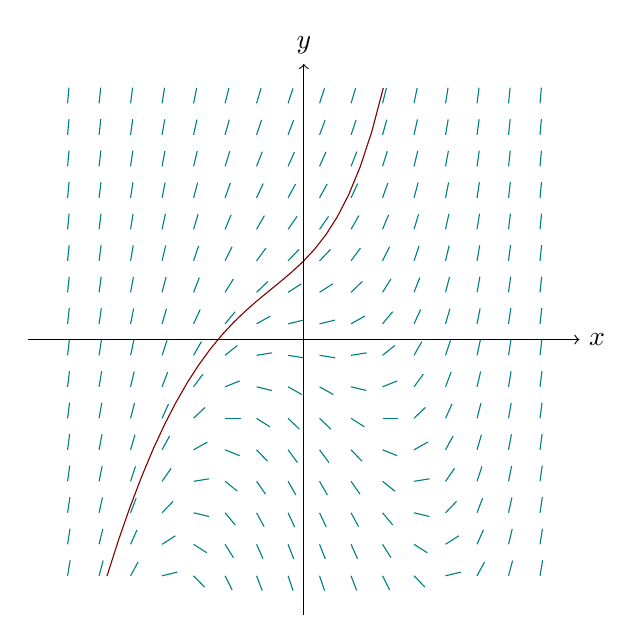
\begin{tikzpicture}[declare function={f(\x,\y)=\x*\x+\y;}]
\def\xmax{3} \def\xmin{-3}
\def\ymax{3} \def\ymin{-3}
\def\nx{15}
\def\ny{15}

\pgfmathsetmacro{\hx}{(\xmax-\xmin)/\nx}
\pgfmathsetmacro{\hy}{(\ymax-\ymin)/\ny}
\foreach \i in {0,...,\nx}
\foreach \j in {0,...,\ny}{
\pgfmathsetmacro{\yprime}{f({\xmin+\i*\hx},{\ymin+\j*\hy})}
\draw[teal, shift = {({\xmin+\i*\hx},{\ymin+\j*\hy})}] 
(0,0)--($(0,0)!2mm!(.1,.1*\yprime)$);
}

% Plot a particular solution passing through y0
\def\y0{1}
\draw[color=Maroon] plot[domain=-2.5:1.01] (\x,{(\y0+2)*exp(\x)-\x * \x - 2 * \x -2});

\draw[->] (\xmin-.5,0)--(\xmax+.5,0) node[right] {$x$};
\draw[->] (0,\ymin-.5)--(0,\ymax+.5) node[above] {$y$};
\end{tikzpicture}
\end{document}